\documentclass{beamer}
\usetheme{Madrid}
\usecolortheme{default}
\usepackage{graphicx}
\graphicspath{{./images/}}
\usepackage{tikz}
\usetikzlibrary{shapes.geometric, arrows.meta, positioning}
\tikzstyle{process} = [rectangle, rounded corners, minimum width=2.5cm, minimum height=1cm,text centered, draw=black, fill=blue!20]
\tikzstyle{arrow} = [thick,->,>=stealth]



\title[SAMASTHA - IELTS MOCK]{SAMASTHA - IELTS MOCK\\\large An AI Powered Preparation Platform}
\author[B Mallesh]{B Mallesh (N190861)}
\institute[RGUKT NUZVID]{Rajiv Gandhi University of Knowledge Technologies\\NUZVID}
\date{}

\begin{document}

%--------------------- Slide 1 ---------------------%
\begin{frame}
  \titlepage
  \begin{center}
    
\includegraphics[width=2.5cm]{images/logo4.jpeg}
  \end{center}
  \vspace{0.3cm}
  \centering
  % \textbf{Guide: Mr. R. Siva Narayana}
\end{frame}


%--------------------- Slide 2 (updated index) ---------------------%
\begin{frame}{Table of Contents}
  \begin{enumerate}
    \item Abstract
    \item Introduction
    \item Related Works / Existing Systems
    \item Proposed Method
    \begin{itemize}
      \item Flowchart
      \item Component Explanation
    \end{itemize}
    \item Technologies Used
    % \item Module-wise Implementation
    % \begin{itemize}
    %   \item Listening
    %   \item Reading
    %   \item Writing
    %   \item Speaking
    % \end{itemize}
    \item Result
    \item Conclusion
    \item References
    \item Project Demo Link
  \end{enumerate}
\end{frame}


%--------------------- Slide 2 ---------------------%
\begin{frame}{Abstract}
  This project implements a comprehensive IELTS examination system that assesses English proficiency through \textbf{Listening, Reading, Writing, and Speaking} modules.

  \vspace{0.2cm}
  It simulates the official IELTS environment, offering realistic practice with timed tests, instant feedback, and performance tracking.

  \vspace{0.2cm}
  Designed for non-native speakers, it supports academic, immigration, and professional needs. The platform emphasizes accessibility, scalability, and a user-friendly interface for diverse users.
\end{frame}

%--------------------- Slide 3 ---------------------%
\begin{frame}{Introduction}
  This IELTS application offers both individual practice tests for each module — \textbf{Listening, Reading, Writing, and Speaking} — as well as full-length tests covering all sections.

  \vspace{0.2cm}
  It provides detailed feedback for each test, maintains test history, and tracks user performance through interactive graphs.

  \vspace{0.2cm}
  The system is designed to help users improve effectively with targeted practice and comprehensive performance insights.
\end{frame}

%--------------------- Slide 4 ---------------------%
\begin{frame}{Related Works / Existing Systems}
  \textbf{Existing Platforms:}
  \begin{itemize}
    \item \textbf{British Council IELTS Prep:} Offers practice tests but lacks real-time feedback and candidate-specific tracking.
    \item \textbf{IELTS Liz / Magoosh:} Focus on content and tips but do not offer interactive test-taking environments or progress analytics.
    \item \textbf{Cambridge IELTS Books:} Provide quality practice material, but are static and not personalized.
  \end{itemize}
  
  \vspace{0.3cm}
  \textbf{Our Differentiation:}
  \begin{itemize}
    \item Designed to train and monitor the progress of candidates who enroll through our service.
    \item Empowers customers (consultants/institutions) to track performance, provide guided improvement, and ensure candidates are exam-ready.
    \item Acts as a bridge between candidates' dreams and actionable, measurable training.
  \end{itemize}
\end{frame}


%--------------------- Slide 5 (Compact Version) ---------------------%
\begin{frame}{Proposed Method - Flowchart}
  \centering
  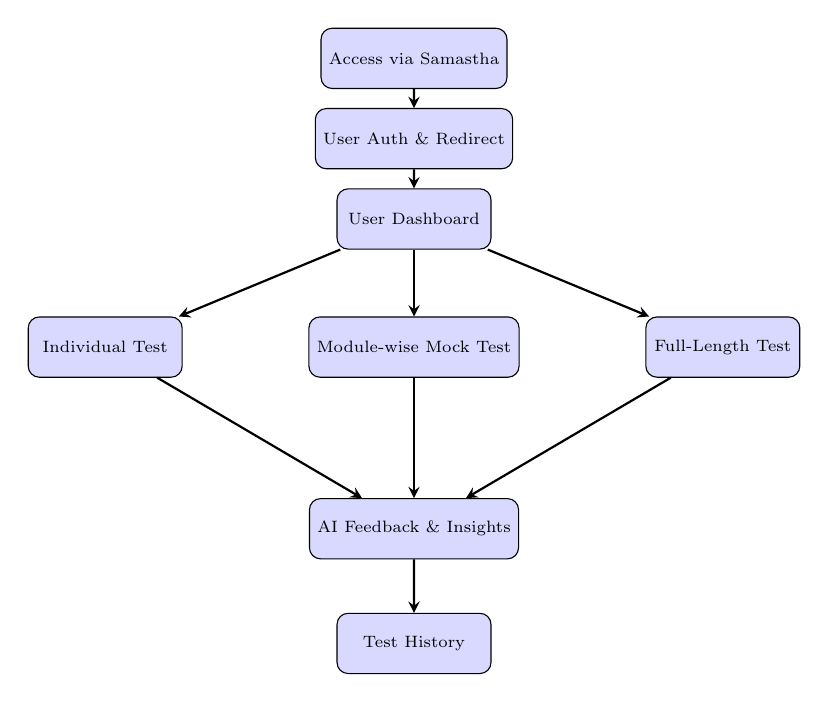
\begin{tikzpicture}[node distance=1.2cm, scale=0.85, transform shape]
    \tikzstyle{smallprocess} = [rectangle, rounded corners, minimum width=2.3cm, minimum height=0.9cm, text centered, draw=black, fill=blue!15, font=\scriptsize]
    
    \node (samastha) [smallprocess] {Access via Samastha};
    \node (auth) [smallprocess, below of=samastha] {User Auth \& Redirect};
    \node (dashboard) [smallprocess, below of=auth] {User Dashboard};

    \node (indTest) [smallprocess, below left=1.0cm and 2.3cm of dashboard] {Individual Test};
    \node (mockTest) [smallprocess, below=1.0cm of dashboard] {Module-wise Mock Test};
    \node (fullTest) [smallprocess, below right=1.0cm and 2.3cm of dashboard] {Full-Length Test};

    \node (aiFeedback) [smallprocess, below=1.8cm of mockTest] {AI Feedback \& Insights};
    \node (history) [smallprocess, below=0.8cm of aiFeedback] {Test History};

    \draw [arrow] (samastha) -- (auth);
    \draw [arrow] (auth) -- (dashboard);
    \draw [arrow] (dashboard) -- (indTest);
    \draw [arrow] (dashboard) -- (mockTest);
    \draw [arrow] (dashboard) -- (fullTest);
    \draw [arrow] (indTest) -- (aiFeedback);
    \draw [arrow] (mockTest) -- (aiFeedback);
    \draw [arrow] (fullTest) -- (aiFeedback);
    \draw [arrow] (aiFeedback) -- (history);
  \end{tikzpicture}
\end{frame}



%--------------------- Slide 6 (Updated) ---------------------%
\begin{frame}{Proposed Method }
  \begin{itemize}
    \item \textbf{Samastha Access:} Users must be registered via the Samastha partner platform. Only verified users can access the IELTS portal.
    
    \item \textbf{User Dashboard:} Central hub for accessing different test types, viewing performance data, and navigating features.
    
    \item \textbf{Test Types:}
    \begin{itemize}
      \item \textbf{Individual Test:} Practice a single part from any module (e.g., a single Listening section).
      \item \textbf{Module-wise Mock Test:} Full mock test of one complete module (e.g., all 3 Reading parts).
      \item \textbf{Full-Length Test:} Simulates the official IELTS exam with all four modules in sequence.
    \end{itemize}
    
    \item \textbf{AI Feedback:} After each test, the system generates detailed, module-specific feedback using AI — covering accuracy, grammar, and suggestions for improvement.
    
    \item \textbf{Test History:} All test attempts are saved with scores and insights, helping users track progress and spot trends over time.
  \end{itemize}
\end{frame}


%------------ Slide: Technologies Used (Images Style) ---------------------%
\begin{frame}{Technologies Used}
  \centering
  \begin{tabular}{ccc}
    
\includegraphics[width=1.8cm]{images/React_logo.png} &
    
\includegraphics[width=1.8cm]{images/tailwind_logo.png} &
    
\includegraphics[width=1.8cm]{images/flask_logo.png} \\
    \small React.js & \small Tailwind CSS & \small Python Flask \\
    \\
    
\includegraphics[width=1.8cm]{images/mySQL_logo.png} &
    
\includegraphics[width=1.8cm]{images/chatGPT_logo.png} &
    
\includegraphics[width=1.8cm]{images/google_Speech_to_text_logo.png} \\
    \small MySQL & \small OpenAI API \& Claude  & \small Google Speech-to-Text \\
    \\
    
\includegraphics[width=1.8cm]{images/JWT_logo.png} &
    
\includegraphics[width=1.8cm]{images/vercel_logo.png} &
    \\
    \small JWT Auth & \small Vercel (Deployment) & \\
  \end{tabular}
\end{frame}


% %--------------------- Slide: Module-wise Implementation (Enhanced) ---------------------%
% \begin{frame}{Module-wise Implementation}
%   The platform supports flexible IELTS preparation through three primary test types:
  
%   \vspace{0.4cm}
%   \begin{itemize}
%     \item \textbf{Individual Tests:} 
%     \begin{itemize}
%       \item Practice a single part from any module (Listening, Reading, Writing, or Speaking).
%       \item Immediate AI-generated feedback after completion.
%       \item Ideal for focused improvement in specific skills.
%     \end{itemize}

%     \vspace{0.2cm}
%     \item \textbf{Module-wise Mock Tests:} 
%     \begin{itemize}
%       \item Attempt an entire module (e.g., all 3 parts of Reading).
%       \item Realistic timing and structure to simulate full module experience.
%       \item Detailed AI feedback covering accuracy, time management, and strategy tips.
%     \end{itemize}
    
%     \vspace{0.2cm}
%     \item \textbf{Full Test Flow:}
%     \begin{itemize}
%       \item Complete IELTS Simulation with all four modules (Listening, Reading, Writing, Speaking) back-to-back.
%       \item Consent pages, Welcome screens, Audio Checks, Instruction pages implemented before starting each module.
%       \item Adaptive timer and navigation controls according to IELTS rules.
%       \item Full AI evaluation report at the end with band score, strengths, omissions, and improvement tips.
%     \end{itemize}
%   \end{itemize}
  
%   \vspace{0.4cm}
%   Test history, performance graphs, and progress tracking are available through the dashboard.
% \end{frame}


%--------------------- Slide: My Work in the Project (1) ---------------------%
\begin{frame}{Result}
  \begin{itemize}
    \item Developed UI using \textbf{React JS} + \textbf{Tailwind CSS} for all modules.
    \item Implemented routing and timer controls for individual and full-length tests.
    \item Designed instruction, question, and result pages with responsive layouts.
  \end{itemize}

  \vspace{0.4cm}
  \centering
  
\includegraphics[width=0.7\linewidth]{images/screenshot_disable.png}
  
  \vspace{0.2cm}
  \tiny Screenshot of Screenshot Disabling Function

  \vspace{0.4cm}
\end{frame}

\begin{frame}{Result}
  \centering
  \includegraphics[width=0.7\linewidth]{images/code_snippet1.png}
  
  \vspace{0.2cm}
  % \tiny Screenshot of Compare Page
    
\end{frame}


\begin{frame}{Result}
  \centering
  \includegraphics[width=0.7\linewidth]{images/code_snippet2.png}
  
  \vspace{0.2cm}
  % \tiny Screenshot of Compare Page
    
\end{frame}

\begin{frame}{Result}

  \centering
  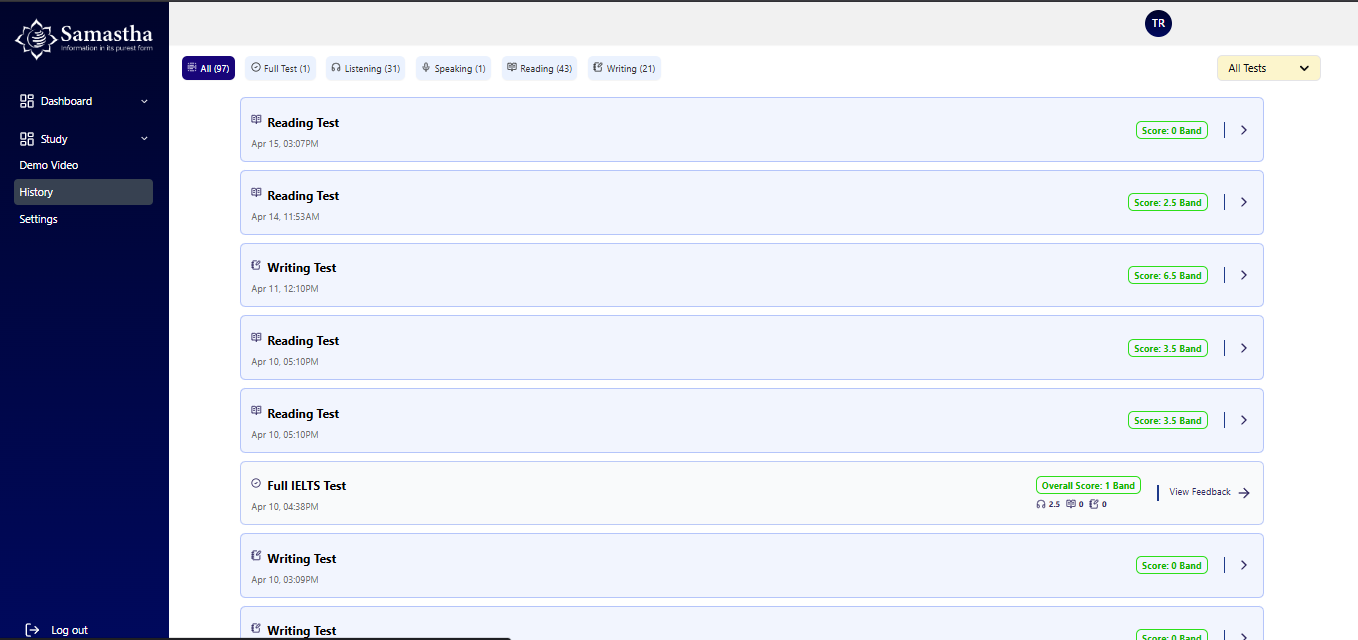
\includegraphics[width=0.7\linewidth]{images/history_page.png}
  
  \vspace{0.2cm}
  \tiny Screenshot of Test History Page
    
\end{frame}

\begin{frame}{Result}

  \centering
  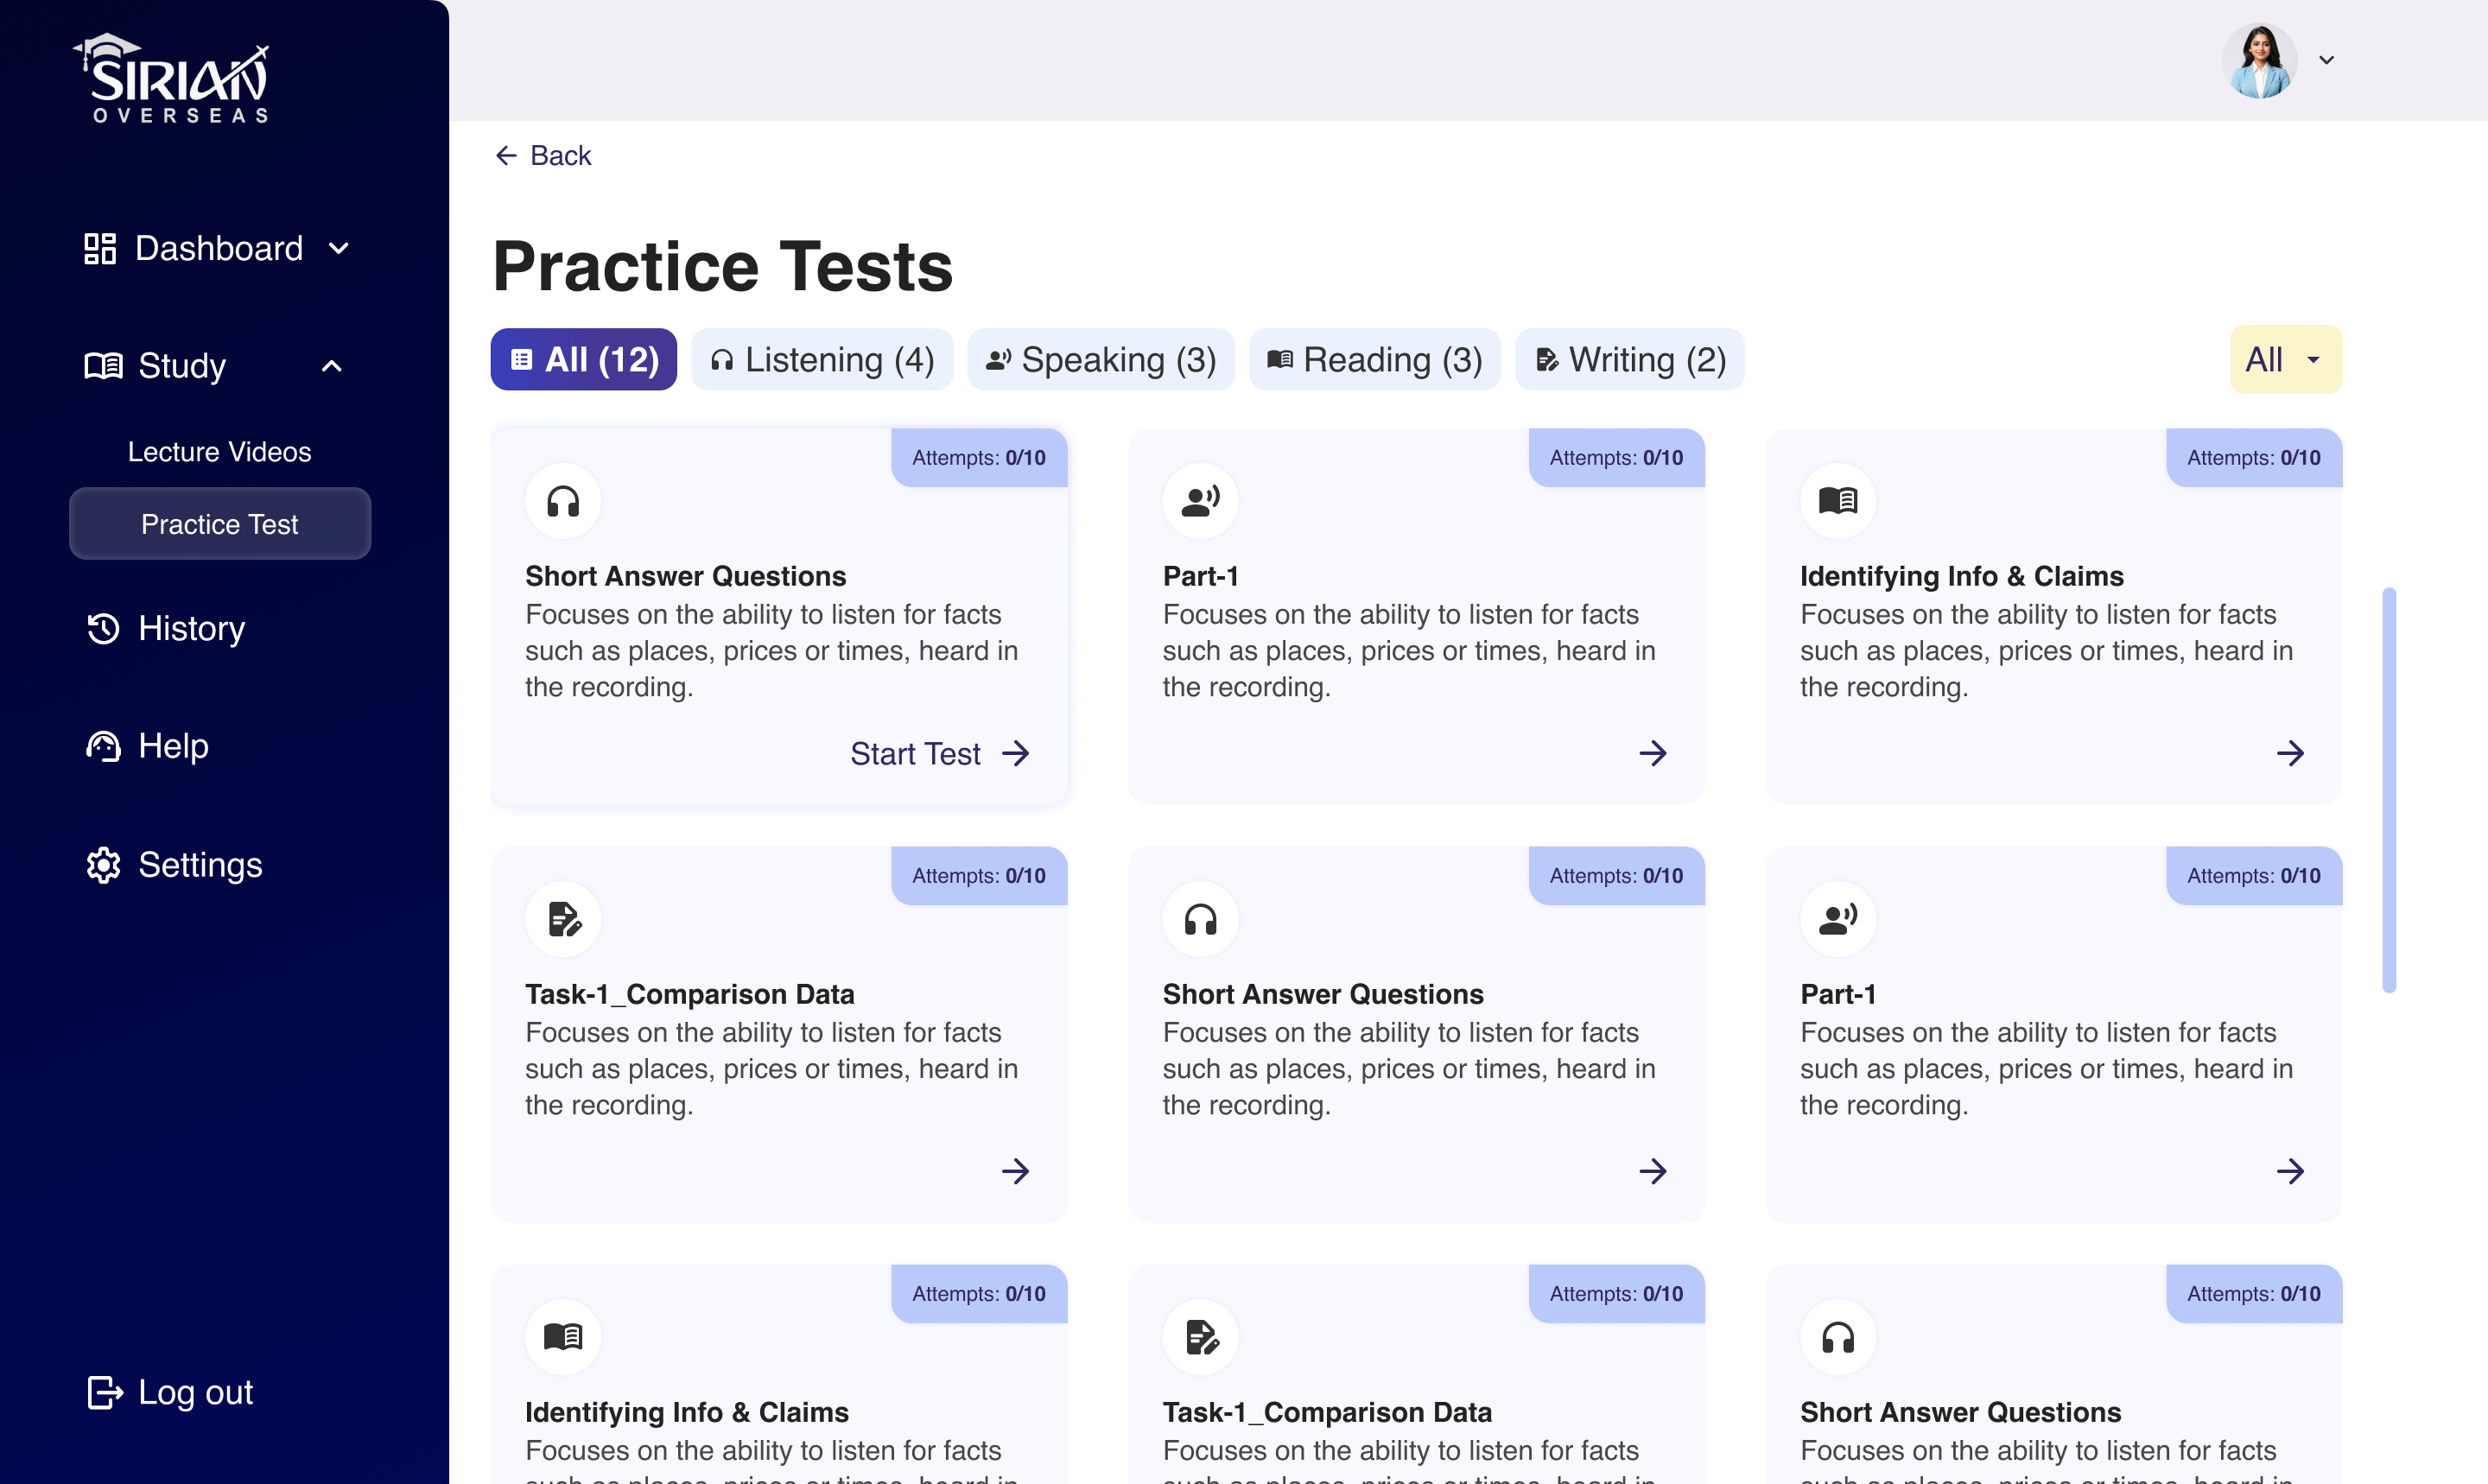
\includegraphics[width=0.7\linewidth]{images/practice_test.png}
  
  \vspace{0.2cm}
  \tiny screenshot of Practice tests cards
    
\end{frame}

\begin{frame}{Result}

  \centering
  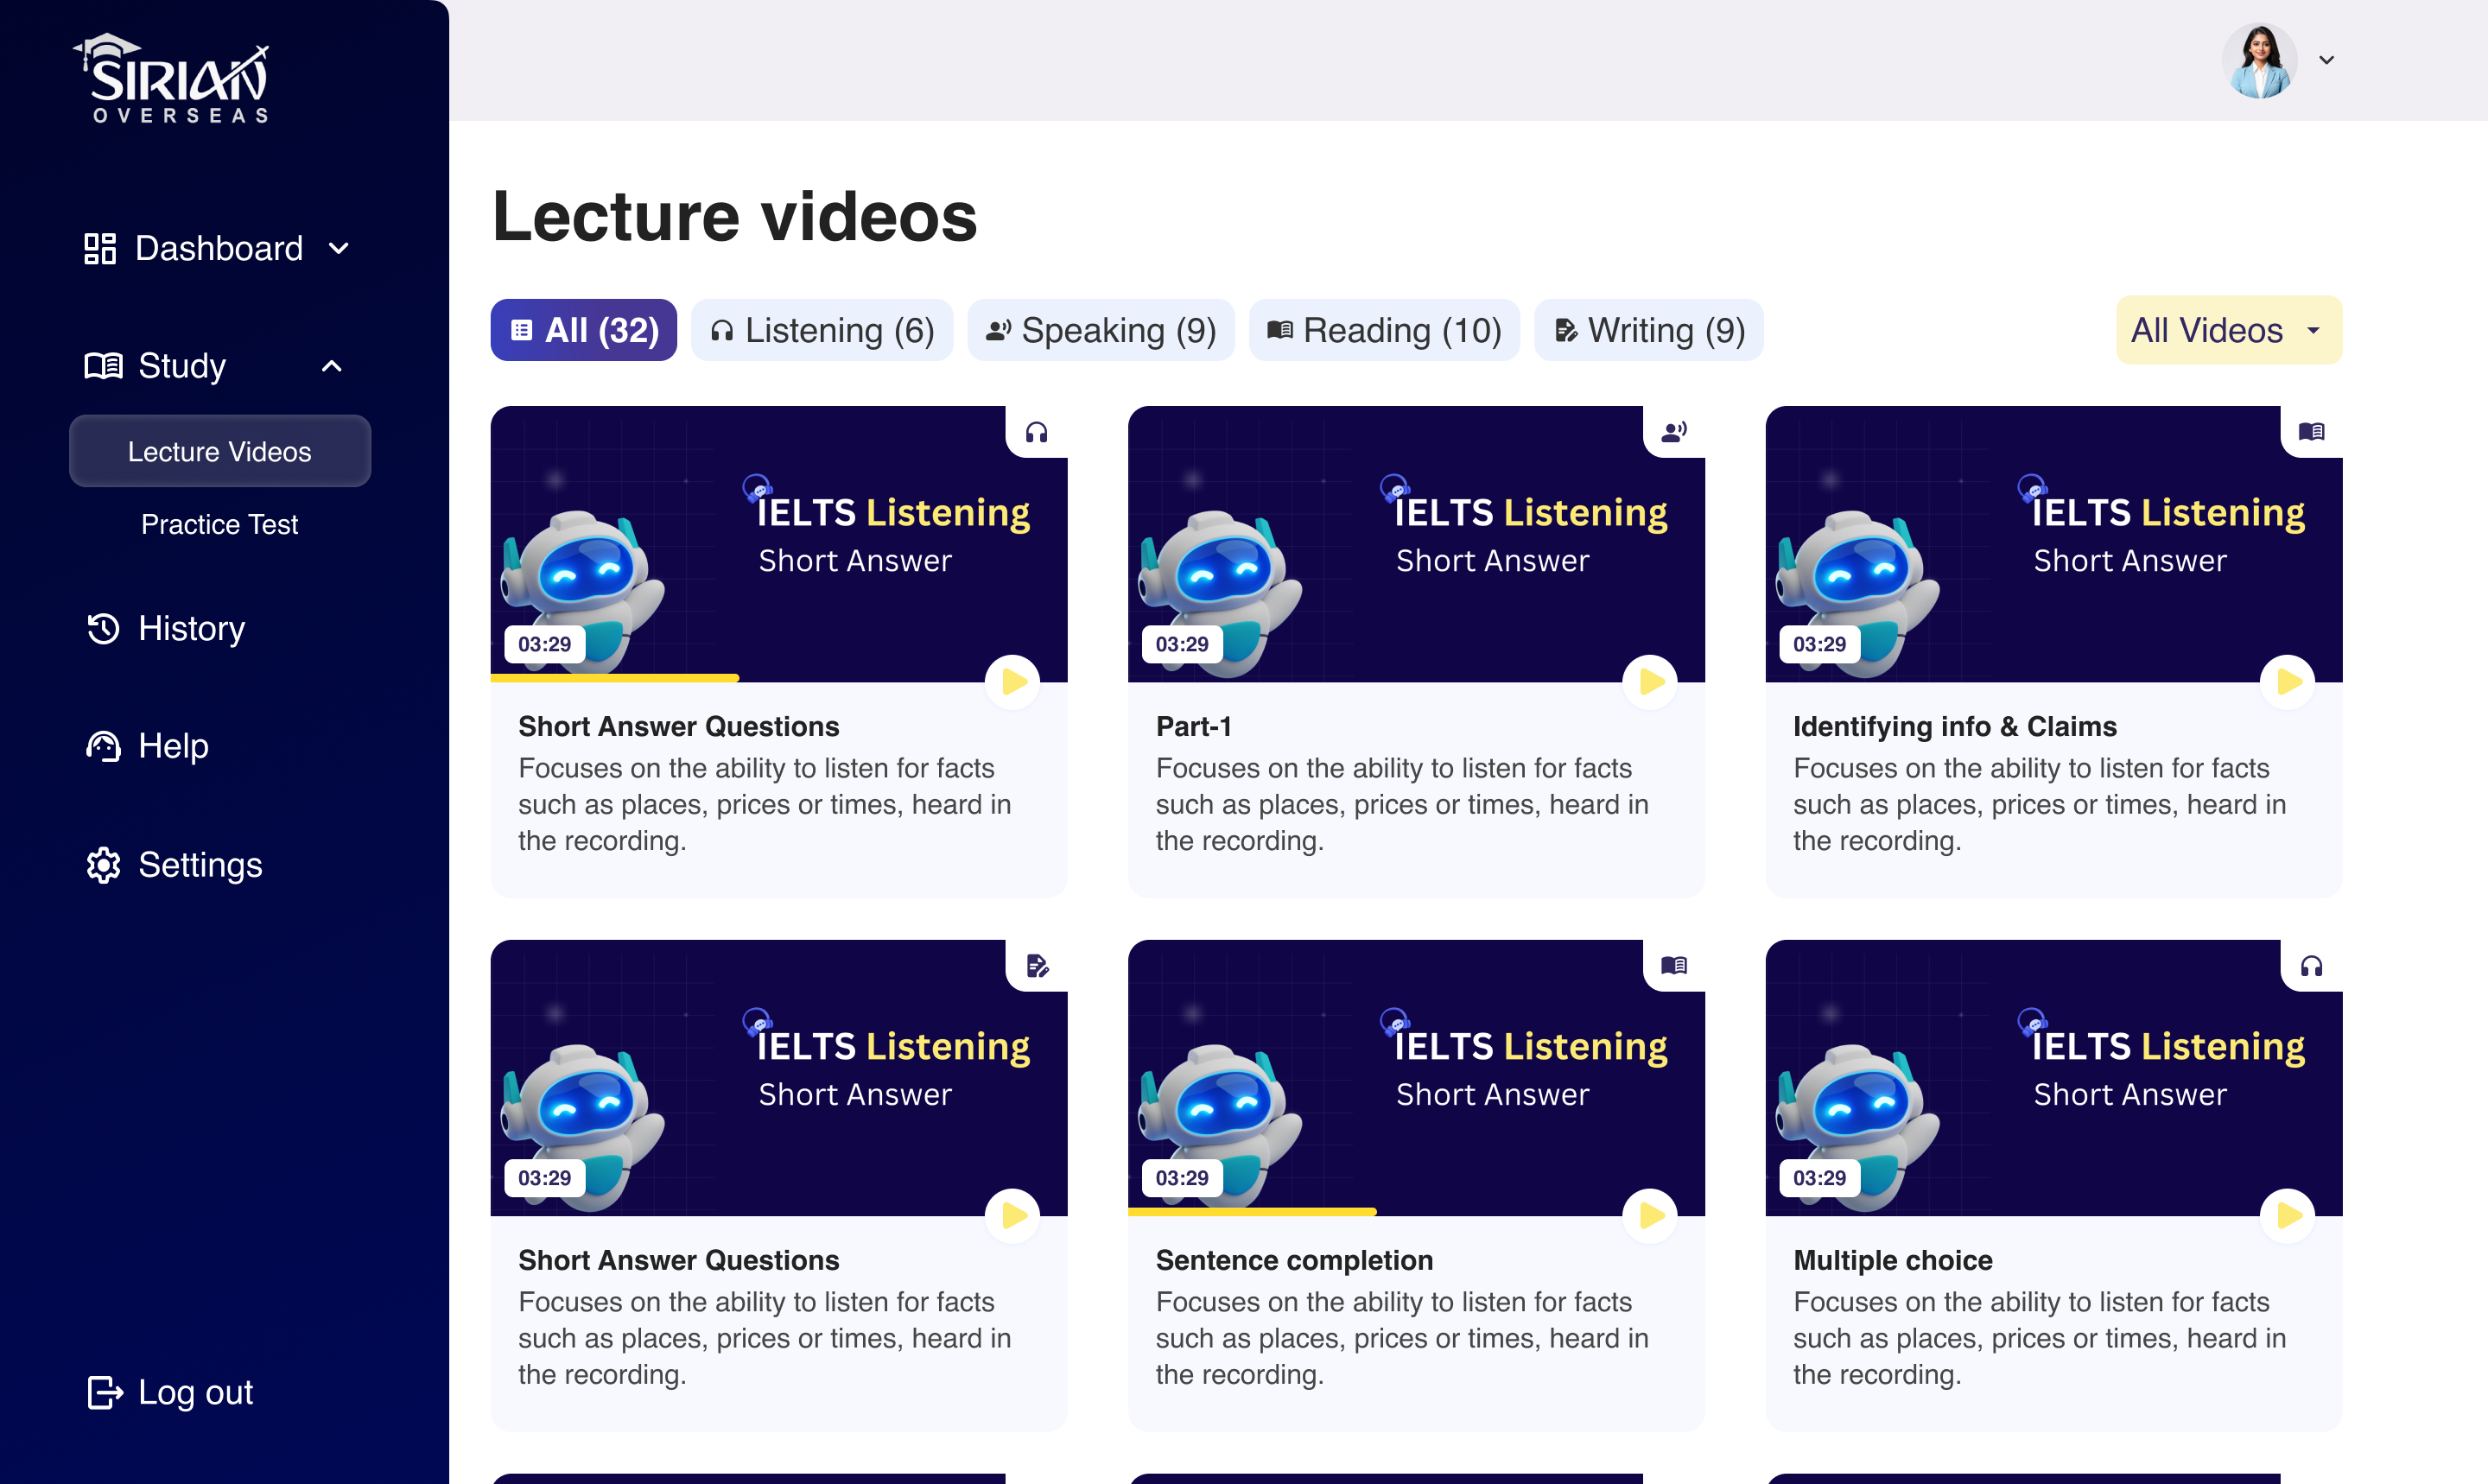
\includegraphics[width=0.7\linewidth]{images/lecture_videos.png}
  
  \vspace{0.2cm}
  \tiny Screenshot of Lecture Videos Page
    
\end{frame}

\begin{frame}{Result}

  \centering
  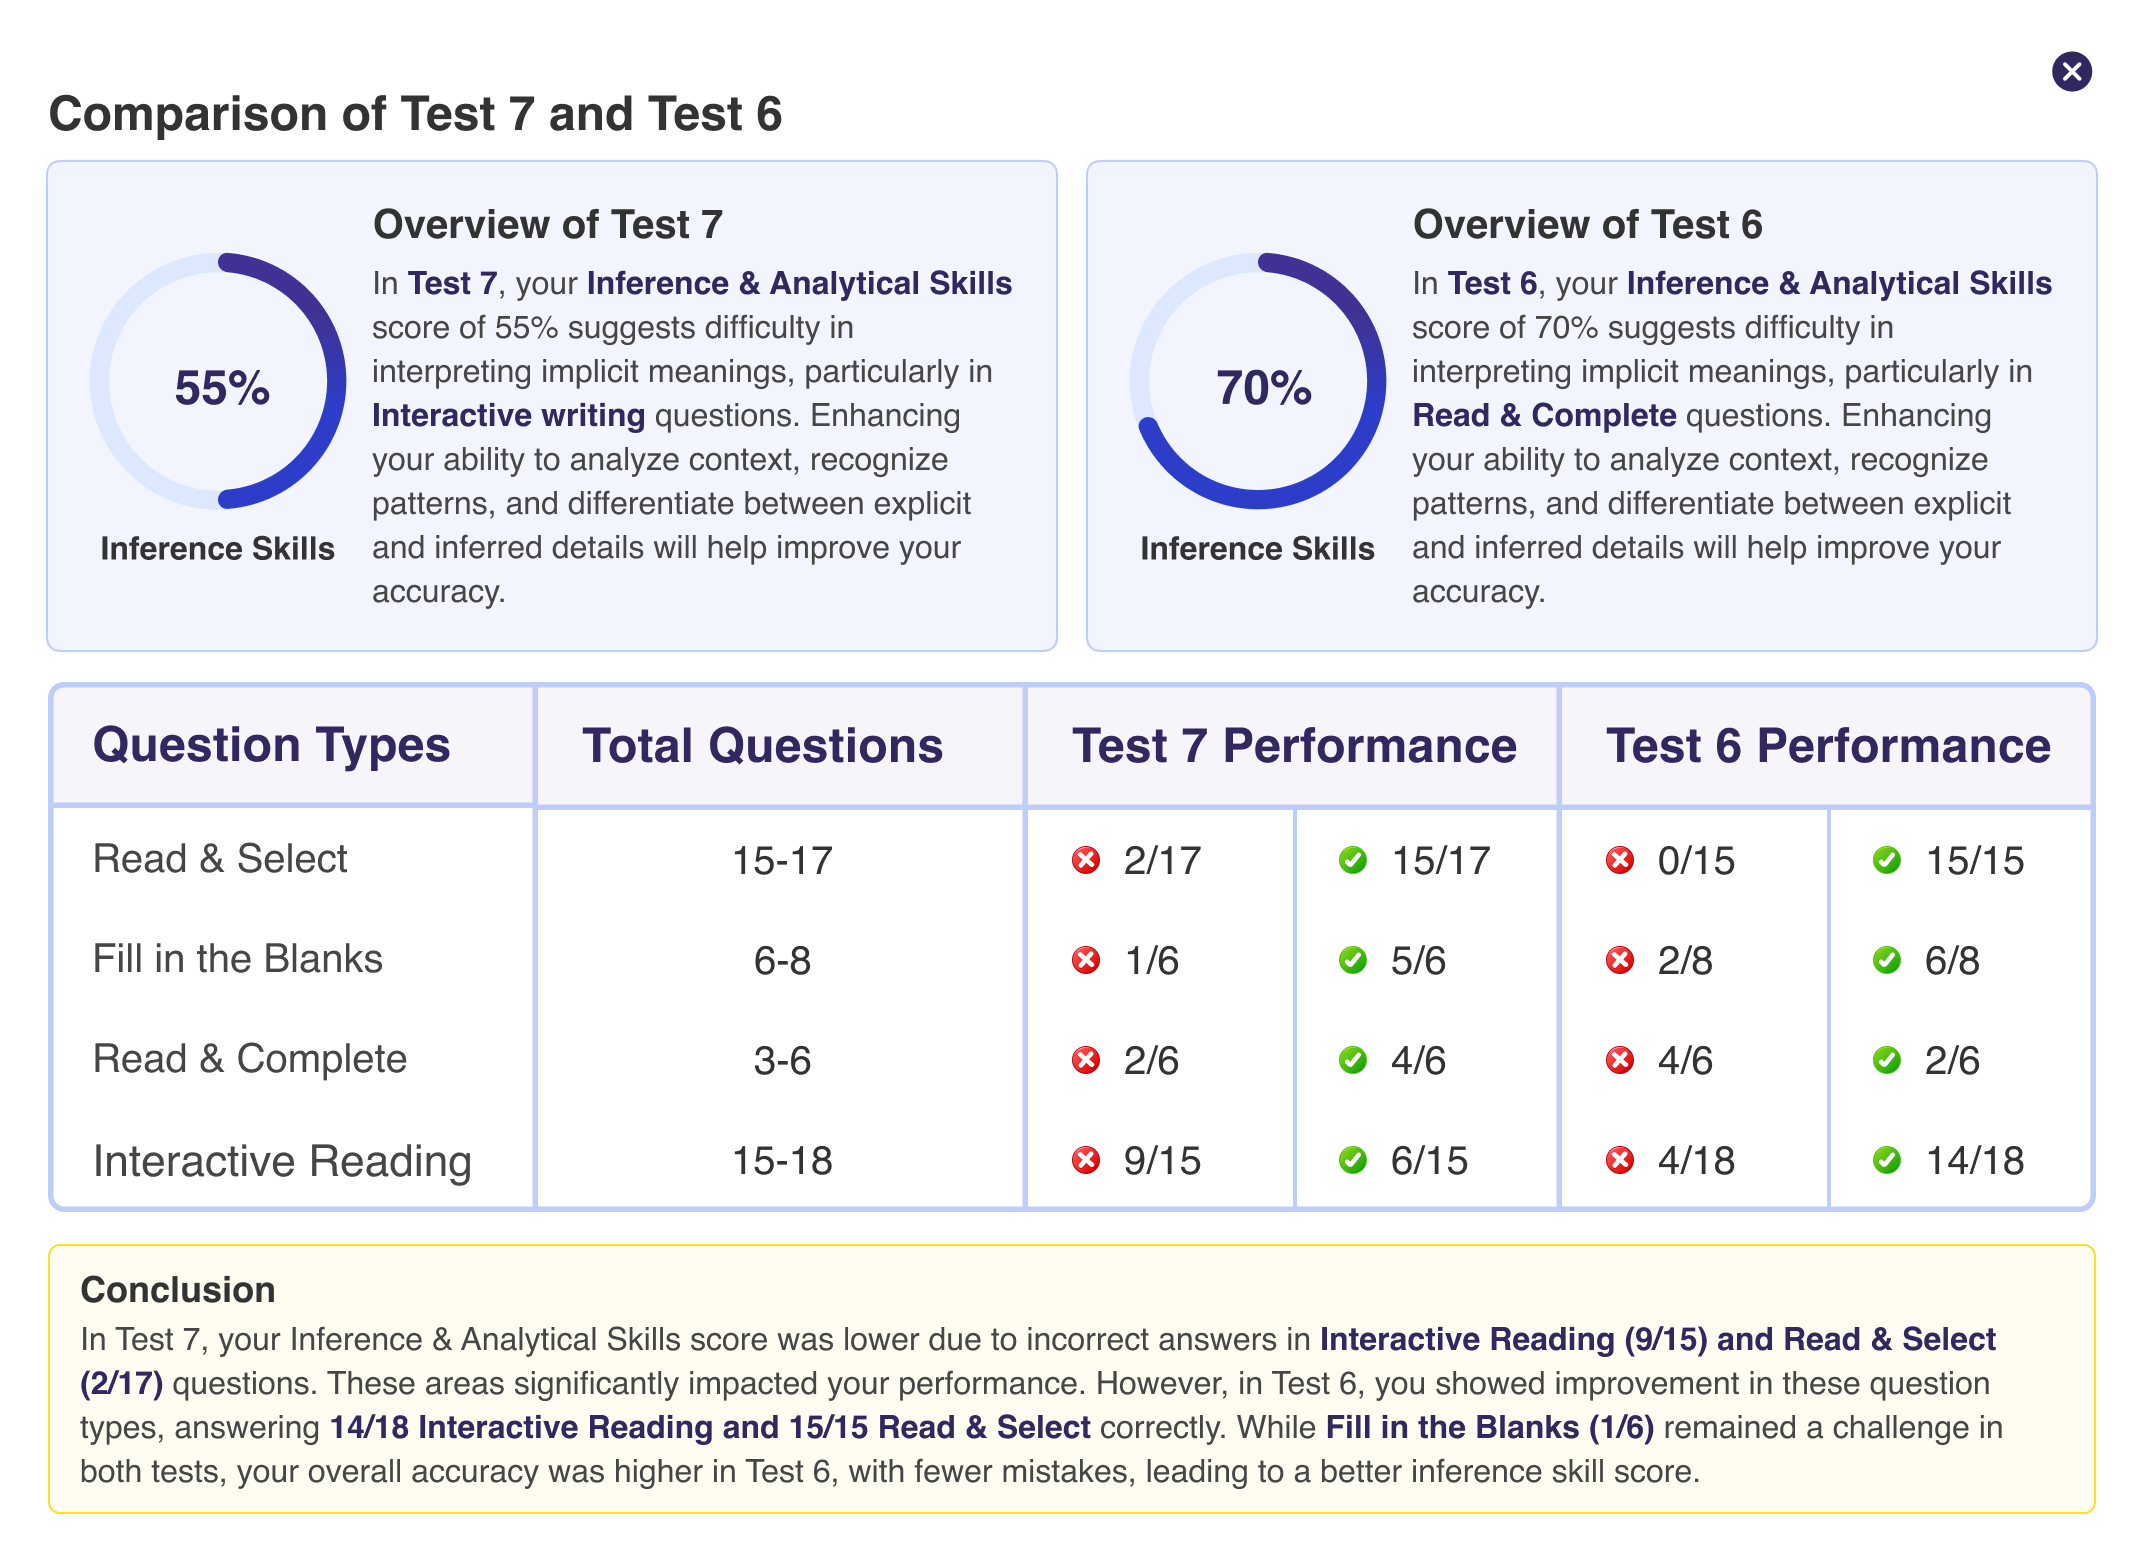
\includegraphics[width=0.7\linewidth]{images/compare_page.png}
  
  \vspace{0.2cm}
  \tiny Screenshot of Compare Page


    
\end{frame}



%--------------------- Slide: Conclusion ---------------------%
\begin{frame}{Conclusion}
  \begin{itemize}
    \item Developed a complete, AI-powered IELTS preparation platform that simulates real exam conditions across all four modules.
    \item Empowered users with dynamic practice environments, instant feedback, and progress tracking dashboards.
    \item Successfully integrated modern technologies such as \textbf{React.js}, \textbf{Tailwind CSS}, \textbf{Python FastAPI/Flask}, and \textbf{AI/NLP services}.
    \item Achieved a seamless, scalable solution for both learners and institutions to enhance English proficiency in a structured, data-driven way.
    \item Future improvements could include mobile app development, peer evaluations, adaptive testing, and LMS integration.
  \end{itemize}
\end{frame}


%--------------------- Slide: References ---------------------%
\begin{frame}{References}

\setbeamertemplate{enumerate items}[square] % <<< THIS FIXES EVERYTHING

\begin{enumerate}
    \item \textbf{Figma UI/UX Design:} \\
    \scriptsize \url{https://www.figma.com/design/9f2Ea52IGTKrhAiZyGWPkn/TEST-PREP-AI-TOOLS?node-id=4943-29809&t=lyBbDLxd5luwzPoH-0}

    \item \textbf{OpenAI API Documentation:} \\
    \scriptsize \url{https://platform.openai.com/docs}

    \item \textbf{Google Cloud Speech-to-Text API:} \\
    \scriptsize \url{https://cloud.google.com/speech-to-text/docs}

    \item \textbf{React.js Official Documentation:} \\
    \scriptsize \url{https://reactjs.org/docs/getting-started.html}

    \item \textbf{Tailwind CSS Documentation:} \\
    \scriptsize \url{https://tailwindcss.com/docs}

    \item \textbf{MySQL Official Documentation:} \\
    \scriptsize \url{https://dev.mysql.com/doc/}

    \item \textbf{Project Contributions and Documentation:} B Mallesh (Self Documentation, Architecture Planning, Final Presentation)
\end{enumerate}

\end{frame}




%--------------------- Slide: Project Demo Link ---------------------%
\begin{frame}{Project Demo}
  \centering
  \textit{"The beautiful thing about learning is that no one can take it away from you."} \\
  \vspace{0.6cm}
  --- B.B. King
  
  \vspace{1.2cm}
  \textbf{Experience the Platform Live:}
  
  \vspace{0.5cm}
  \url{https://www.samasthabroad.com}
  
  \vspace{1.5cm}
  \textbf{Thank You!}
\end{frame}




%----------------------------------------------------------------%
\end{document}
